
\newcommand{\figurewidth}[0]{1.8in}

\newcommand{\tablefig}[1]{
  \hspace*{-0.25in}
  \includegraphics[width=\figurewidth]{../graphs/graphs/#1}
}

\begin{figure}
\begin{center}
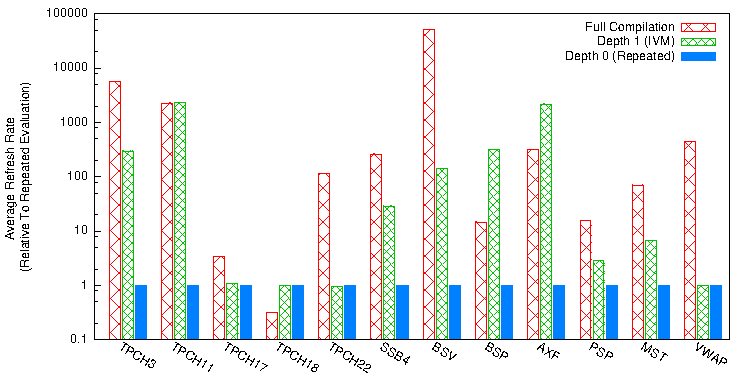
\includegraphics[width=3.4in]{../graphs/graphs/bakeoff.pdf}
\caption{Performance improvement achievable by our compiler.  Note the logscale on the y-axis.  Detailed results for each query are presented below.}
\label{fig:experiments:bakeoff}
\end{center}
\vspace*{-0.2in}
\end{figure}

\begin{figure}
\begin{center}
\resizebox{3.3in}{!}{
\begin{tabular}{|r|cccc|}\hline 
Query & Full Compilation & Depth 1 & CSPE & CDB\\ \hline 
{\bf TPCH3} & 27342.14 & 4.75 & 59.69 & 38.34\\ \hline 
{\bf TPCH11} & 44597.8 & 19.51 & XXX & XXX\\ \hline 
{\bf TPCH17} & 66.27 & 19.76 & 32.58 & 8.48\\ \hline 
{\bf TPCH18} & 1.95 & 6.13 & 21.13 & 38.07\\ \hline 
{\bf TPCH22} & 273.37 & 2.4 & 39.82 & 45.83\\ \hline 
{\bf SSB4} & 50.4 & 0.19 & 69.19 & 103.29\\ \hline 
{\bf BSV} & 110261.68 & 2.18 & XXX & XXX\\ \hline 
{\bf BSP} & 9.24 & 0.63 & 13.79 & 31.47\\ \hline 
{\bf AXF} & 54.15 & 0.17 & 12.28 & 31.1\\ \hline 
{\bf PSP} & 10.69 & 0.67 & 10.52 & 13.32\\ \hline 
{\bf MST} & 9.1 & 0.13 & 7.51 & 30.88\\ \hline 
{\bf VWAP} & 3259.47 & 7.4 & 9.31 & 12.89\\ \hline 
\end{tabular}
}
\caption{Comparison between the performance of our compiler and the two commercial data processing engines (in \# of refreshes per second) from Section \ref{sec:sota}.  These engines are performing the same amount of work as depth-0, and their performance improvement over it is the result of extensive optimization.  We expect a similar level of improvement to be possible for full compilation.}
\label{fig:experiments:enginesVsDBT}
\vspace*{-0.3in}
\end{center}
\end{figure}

We now analyze the performance of our compilation techniques.  As in Section \ref{sec:sota}, our experiments are run on Redhat Enterprise Linux running in a VM with 16 GB of RAM, and 2x4 core Intel Xeon E5620 2.4 GHz processors allocated to it.  Note that our compiler produces single-threaded code, while other platforms were allowed to consume the full resources of the VM.

Our analysis uses the same queries and methodology as in Section~\ref{sec:tscomparison}: The queries are described in Section~\ref{sec:tscomparison:workload}, and expressed in SQL form in Appendix~\ref{app:queries}.

Memory measurements are taken using google-perftools\cite{perftools}, and count only memory allocated to the persistent maps and not transient datas (e.g., materialized join results).  

% we analyze our compiler's performance on TPC-H\cite{tpch} Queries 3, 11, 17, 18, and 22, a variant of Star Schema Benchmark\cite{ssb} Query 4 six orderbook queries: VWAP, PS, MST, AXF, BSP, and BSV, and a cluster monitoring query: SVL.  TPC-H queries were modified slightly due to a lack of support for certain advanced features in our SQL parser (e.g., Having, Exists, etc...).  SQL for the queries in our test workload is presented in Appendix

%Our analysis uses the queries from Examples \ref{ex:dbfail:stock} (PS),  \ref{ex:dbfail:tpch} (SSB4), and \ref{ex:dbfail:network} (SVL), Queries numbers 3, 11, 17, 18, and 22 from the TPC-H\cite{tpch} benchmark, the VWAP query presented in \cite{kennedy-ahmad-koch-cidr:11}, and four additional financial queries: MST, AXF, BSP, and BSV in the spirit of VWAP and PS.  The structure of these queries is discussed below.

Queries were run on pre-generated traces until completion of the trace or a 1 hour cutoff was reached -- overall rates are computed based on the number of tuples completed after 1 hour.  Traces were generated as follows: The queries: VWAP, MST, AXF, BSP, PS, and BSV were run on a 2.63 million tuple trace of an order book update stream, representing of one day of stock market activity for MSFT.  BID and ASK orders (and cancellations) were translated into equivalent operations on a BIDS and ASKS table, with tuples in either table comprised of a timestamp, an order id, a broker id, a price, and a volume.  The broker id was synthesized for each order -- our experiments use 10 brokers, assigned deterministically based on the order id.  The stream consists of approximately 1.4 million operations on the BIDS table, and 1.14 million operations on the ASKS table.

Queries based on the TPC-H schema (including SSB4) were run on a scaling-factor 0.1 (100 BM) database generated by dbgen\cite{counciltpc}.  Additional scaling experiments were carried out on TPC-H queries 3 and 11 at scaling factors 0.5, 1, 5, and 10 -- these results are presented in Section~\ref{sec:experiments:bigds}.  Insertions are drawn in-order from each output file of dbgen, with rows from different tables interleaved in random order.  Note that it possible for rows to be inserted before a foreign key constraint has been satisfied, and that smaller datafiles will finish earlier in the stream.  This is not expected behavior in a streaming setting, but provides valuable insights about the performance characteristics of insertions into different tables.

%SVL was run on a synthetically generated dataset, simulating 1000 racks of 20 servers each, emitting a total of 100,000 state updates.  The first 20,000 operations in the trace consist of an insertion for each server at 0 load.  For each state update, a random server deletes its previous state tuple and inserts a tuple declaring its new load -- a random real between 0 and 1.

In order to evaluate our compilation algorithm in a fair environment with a common baseline for performance, we use a depth-limited instantiation of our compilation algorithm: Instead of recursively computing the entire materialization plan, the compiler stops after a fixed number of recursive steps.  Beyond this stage, queries are not materialized and instead computed directly from the base relations.   Compilation at depth-1 is equivalent to traditional IVM techniques, and depth-0 is equivalent to re-evaluating the query on every insertion.  Figure \ref{fig:experiments:bakeoff} illustrates, at a high level, the results of these comparisons.

As a consequence of the high join width of SSB4, the default materialization plan has an extremely high branching factor (12 at the top level).  Although most materialized views in the plan are duplicates, the compiler must still explore all children of unique nodes -- a prohibitively expensive process.  For the purpose of these experiments, we omit deletions when compiling SSB4 (halving the branching factor).  As SSB4 is a query without nested aggregates, deletions are symmetric with insertions -- In spite of the prohibitive compilation time, the behavior of the compiled query is identical.

\tinysection{Comparison with Existing Systems}
Figure \ref{fig:experiments:enginesVsDBT} compares our recursive compilation technique to the performance of the traditional databases and stream processors presented in Section~\ref{sec:sota} (and Figure~\ref{fig:queries}).  Recall that CSPE is implemented using IVM techniques, while CDB uses repeated evaluation.  CDB's performance with respect to our depth-0 evaluation implementation bodes well for our techniques.  It is reasonable to expect that at least order of magnitude gain in the performance of full compilation can be achieved through a commercial-grade level of performance tuning.

\subsection{Equijoins}

We first analyze the performance of our compiler on three equijoin queries with no nested aggregates.  Our compiler recurs only once on TPCH11.  As a consequence, the result is nearly equivalent to IVM.  We pre-aggregate the materializations of SUPPLIER and PARTSUPP, but this provides only a minor improvement at this scale\footnote{Note however the results of Figure~\ref{fig:experiments:big}b.}.  

Both TPCH3 and SSB4 demonstrate a substantial performance increase over IVM.  The one-to-one, and bounded fanout one-to-many relationships between elements of many of these queries are actually advantageous to the IVM implementation -- each insertion only triggers a limited number of reads.  In spite of this, incrementally maintaining the (aggregate) delta queries results in a net reduction in the amount of work required -- especially in a large query like SSB4.

Also note the memory usage of TPCH3.  Starting by the 40\%\ marker, all streams have been exhausted except for LINEITEM.  The final aggregate's group-by columns are drawn purely from the order table, so insertions into LINEITEM only update aggregate values that have already been allocated by the corresponding ORDER.  Thus, memory usage plateaus for full compilation, while the IVM implementation must continue to store each row.

This is not always true.  For extremely large queries like SSB4 (a 7-way join), the number of intermediate materialized views created is quite large.  Despite the large amount of state that the fully compiled query maintains, any individual update modifies only a small amount of that state, and the fully compiled query's efficiency is unaffected as long as the system has enough memory.  However, memory usage is an important part of the cost/benefit tradeoff of full compilation -- We address a broader range of materialization strategies below in Section~\ref{sec:experiments:othermetrics}.



\begin{figure*}
\begin{center}

\begin{minipage}{\textwidth}
\begin{center}
\hspace*{0.1in}
\begin{tabular}{cccc}
\tablefig{unified_tpch3.pdf} &
\tablefig{unified_tpch11.pdf} &
\tablefig{unified_tpch17.pdf} &
\tablefig{unified_ssb4.pdf} \\
(a) & (b) & (c) & (d)
\end{tabular} \vspace*{-0.2in}
\caption{TPCH3~(a), 11~(b), 17~(c), and SSB4~(d): (a) By the 40\%\ marker, all streams except LINEITEM have completed, and the remaining tuples consume no additional memory. (b) For simple two-way joins, full compilation is virtually identical to depth-1 and takes under 2 seconds, while depth-0 takes over an hour. (c) Due to the nested aggregate, IVC requires a nested loop, while full compilation requires only a single scan. (d) Full compilation is a full polynomial order faster than in IVC, although performance does begin to drop once the system begins running out of memory around the 27\%\ marker.}
\label{fig:experiments:tpch3}  
\label{fig:experiments:ssb4}
\label{fig:experiments:tpch17}
\label{fig:experiments:tpch11}
\end{center}
\end{minipage}

\vspace*{0.1in}

\begin{minipage}{\textwidth}
\hspace*{0.1in}
\begin{tabular}{cccc}
\tablefig{unified_brokervariance.pdf} & 
\tablefig{unified_vwap.pdf} &
\tablefig{unified_tpch18.pdf} &
\tablefig{unified_tpch22.pdf} \\
%\tablefig{unified_serverload.pdf} \\
(a) & (b) & (c) & (d)
\end{tabular} \vspace*{-0.2in}
\caption{BSV~(a), VWAP~(c), TPC-H Queries 18~(b), and 22~(d):  (a) The many-to-many relationship on the join term forces IVM to perform linear work on each insertion, which full compilation avoids. (b) IVM repeatedly re-evaluates the nested (parameterized) sub-query, while full compilation maintais a cache of sub-query results. (c): TPCH18 An badly chosen join ordering prevents full compilation from effectively exploiting foreign key dependencies in the TPC-H schema. (d) The small CUSTOMER stream completes at the 10\%\ marker, while the remaining ORDERS tuples require only linear time with full compilation. }


%(d) Materializing nested queries gains a polynomial degree of performance over IVM, but memory continues to grow. 
\label{fig:experiments:brokervariance}
\label{fig:experiments:tpch22}
\label{fig:experiments:vwap}
\label{fig:experiments:tpch18}
\label{fig:experiments:serverload}
\end{minipage}

\vspace*{0.1in}

\begin{minipage}{\textwidth}
\hspace*{0.1in}
\begin{tabular}{cccc}
\tablefig{unified_pricespread.pdf} &
\tablefig{unified_missedtrades.pdf} &
\tablefig{unified_axfinder.pdf} &
\tablefig{unified_brokerspread.pdf} \\
(a) & (b) & (c) & (d)
\end{tabular} \vspace*{-0.2in}
\caption{PS~(a), MST~(b), AXF~(c) and BSP~(d):  (a,b) The performance and memory plateaus result from a portion of the trace from about 0.001\%\ to 0.01\%, where a single order is repeatedly placed and revoked. (c,d) Full compilation's aggressive materialization strategy results in the caches growing too large to be efficiently maintained.}
\label{fig:experiments:pricespread}
\label{fig:experiments:missedtrades}
\label{fig:experiments:axfinder}
\label{fig:experiments:brokerspread}
\end{minipage}

\end{center}
\end{figure*}


\subsection{Nested Subqueries}

Figures \ref{fig:experiments:tpch17}c, \ref{fig:experiments:vwap}b, and \ref{fig:experiments:tpch22}d illustrate the performance of our compiler on several queries with nested aggregates.

The lookup over ORDERS in TPCH22 can be evaluated in constant time both using IVM and full compilation.  However each insertion into ORDERS requires evaluating the nested aggregate on CUSTOMER, while full compilation materializes the aggregate result instead.

In IVM, insertions into CUSTOMER depend on whether the query optimizer detects that the nested aggregate is uncorrelated and computes it before the rest of the query.  If not, the insertion requires quadratic work, and even if it does, each insertion requires two complete iterations over the customer table: once to compute the aggregate and once to figure out for which customers the state of the comparison changes.  This latter iteration can not be eliminated by full compilation, but the iteration is only over those rows already known to satisfy the selection condition on ORDERS.

VWAP is a query over BIDS with two selection predicates: one over an uncorrelated nested aggregate over BIDS, and one over a correlated (via inequality on the price from the outer BIDS table) nested aggregate over BIDS.  

As with TPCH22, VWAP's uncorrelated aggregate can be evaluated efficiently if the query optimizer spots it -- the inequality-correlated aggregate is of more interest.  Because the domain of the correlating variable (price) is determined outside the nested aggregate, the nested subquery must be re-evaluated every time a new price is encountered.  However, the aggregate value can then be stored and incrementally maintained from that point on.  The domain of prices is bounded, so after an initial ramp up process (that occurs while the size of the table is small) the fully compiled version can incrementally maintain the query output in (close to) constant time.

THe performance of BSV (Figure \ref{fig:experiments:brokervariance}a) is similar to the prior two queries.  This is not surprising -- correlated aggregate subqueries are known to be equivalent to joins, and materializing a nested aggregate is tantamount to materializing the first delta.  Furthermore, unlike TPCH11 (Figure \ref{fig:experiments:tpch11}d), the join relationship is many-to-many, and the benefits of maintaining the join result as an aggregate grow over time.

As in the last several queries, incrementally maintaining the nested aggregate of TPCH17 makes insertions into PART constant-time rather than linear.  Even in the fully compiled version, insertions into the LINEITEM table must still iterate over the results of the join -- under full compilation this join has already been materialized.
%
%\subsection{5 GB Dataset}
%\ref{sec:experiments:bigds}
%Figure \ref{fig:experiments:big} presents the behavior of the three fastest TPC-H queries on a scaling factor 5 (5 GB) database.
%
%In the IVM version of TPC-H 3, the one-to-many relationship between them makes each insertion into CUSTOMER linear in the number of LINEITEMS matching CUSTOMER (an average fanout of 40).  A small CUSTOMER table can be processed before many ORDERS are inserted.  With the larger dataset, the increasing cost of insertions into CUSTOMER becomes more pronounced, while the fully compiled version remains constant-time throughout.
%
%Although IVM is nearly identical to full compilation on TPC-H 11, full compilation pushes aggregation into the materialized view while IVM performs the aggregation at lookup.  This, when inserting into SUPPLIER, full compilation reads precisely one value, while IVM reads approximately 80 (and must aggregate over them).  IVM stores both base relations in their entirety, while full compilation stores only the subset needed for query maintenance.  As a consequence, full compilation has a constant, but visible improvement in both performance and memory use at this scale.
%
%Under full compilation, TPCH22 requires a linear amount of work for insertions into CUSTOMER and a constant amount of work for insertions into ORDERS.  On the small dataset, full compilation was able to get through the CUSTOMER table (note the quadratic behavior in Figure \ref{fig:experiments:tpch22} up to about the 18\% marker) and quickly completed the much larger ORDERS table.  On the larger dataset, full compilation gets bogged down in processing CUSTOMER.

\subsection{Other Metrics}
\label{sec:experiments:othermetrics}

\tinysection{Limited Recursion}
\begin{figure}
\begin{center}
\resizebox{3.4in}{!}{
\begin{tabular}{|l|c|c|c|c|c|c|}\hline
{\bf Depth} & 1 & 2 & 3 & 4 & 5 & Full \\ \hline 
Avg Rate (refreshes/s) & 5.91 & 0.373 & 0.7 & 12.7 & 51.5 & 50.4 \\ \hline 
Avg Memory per Tuple & 98.5 B & 0.0 B & 0.0 B & 0.0 B & 0.0 B & 61.0 KB \\ \hline 
Lines of Code & 3174 & 12015 & 16517 & 13215 & 10998 & 10431 \\ \hline 
Number of Maps &        6 &       18 &       36 &       45 &       45 &       39 \\ \hline 
\end{tabular}
}
\caption{Statistics for different compilation depths on SSB4.  Depth-5 is equivalent to full compilation, but also maintains copies of each of the 6 base relations.}
\label{fig:experiments:ssb4depth}
\end{center}
\vspace*{-0.2in}
\end{figure}
We now explore the space of limited recursive compilation beyond IVM.  Figure \ref{fig:experiments:ssb4depth} illustrates the effects of limiting compilation to depths between 0 and 5.  Recall that the maximum recursive depth is one less than the join width of the query.  Thus for SSB4 (which has a join width of 6), compilation to depth-5 is equivalent to full compilation, save that the base relations are maintained and materialized.

At depth-1, the compiled query materializes only the base relations and no intermediate tables.  It must still perform a 5-way join on every insertion, but  only once per update.  The 6 materialized views that it maintains are the 6 base relations from the query.  

At depth-2, the compiled query must now maintain 12 intermediate materialized views, several of which require (effectively) a 4-way join to maintain.  The net cost of maintaining these additional maps does not begin to pay off until depth-4 (where maintenance operations are reduced to at most 2-way joins).  By this point, decomposition has already resulted in the instantiation of all intermediate materializations relevant to the query, so extra and unnecessary work is being done.  

The effectiveness of this approach at depth-4 (in spite of the extra work being done) suggests that a more effective approach to reducing memory consumption might be to materialize not just the set of views closest to the root, but rather a subset of the entire materialization plan (e.g., requiring at most two-way joins throughout the materialization plan).  However, there exists an incredibly large space of possible materialization plans ($2^{39} \approx $ half a trillion possibilities for SSB4) -- cost based optimization within the space of possible materialization plans is future work.

\tinysection{Scaling}
We now consider the performance scaling of the two best-performing TPC-H Queries (3 and 11) on larger datasets, as presented in Figure \ref{fig:experiments:big}.  The IVM implementation does not complete any workload for Query 3 for any scaling factor.  With full compilation, Query 3 consumes a large fraction of system memory on the 10 GB dataset, but performance remains constant throughout.  Query 11's performance also remains constant -- note the nearly 50\% improvement over IVM at higher scales, an effect of pushing aggregation into the materialized views.

\tinysection{Functional Optimizations}
\todo{Yanif}

\subsection{Memory, Extraction, and Future Work}
\label{sec:experiments:future}

\begin{figure}
\begin{center}
\begin{tabular}{|l|c|c|c|}\hline 
\ & Infinite Depth & Depth 1 & Depth 0 \\\hline 
TPCH3 & 2509 & 2855 & 4198 \\\hline
TPCH11 & 531 & 596 & 616 \\\hline
TPCH17 & 928 & 1158 & 1478 \\\hline
TPCH18 & 3668 & 3538 & 4631 \\\hline
TPCH22 & 777 & 1135 & 754 \\\hline
SSB4 & 10995 & 8954 & 7904 \\\hline
BSV & 342 & 327 & 347 \\\hline
BSP & 45625 & 567 & 729 \\\hline
AXF & 2169 & 553 & 1394 \\\hline
PSP & 1442 & 1878 & 1890 \\\hline
MST & 5457 & 2870 & 2434 \\\hline
VWAP & 533 & 466 & 341 \\\hline
\end{tabular}
\caption{Lines of C++ Code Generated for each}
\label{fig:experiments:loc}
\end{center}
\vspace*{-0.2in}
\end{figure}

It is important to understand not only where our compiler succeeds, but where its limitations lie.  We now consider several cases where the observed performance of our technique does not match up with our (high, and perhaps naive) expectations.  As a consequence of our experimentation and analysis, we have identified three core challenges for future work in this area.

\tinysection{Join Ordering}
In spite of the simplicity of TPCH18 (Figure \ref{fig:experiments:tpch18}b), the query performs poorly -- even repeated evaluation is faster.  This is a consequence of our join ordering heuristic: The trigger that updates the query result must compute a join between the delta of the extracted nested subquery (aggregated over orderkey) and a materialized representation of CUSTOMER $\bowtie$ ORDER $\bowtie$ LINEITEM (aggregated over custkey and orderkey).  

Not knowing about the one-to-many relationship between custkey and orderkey, we iterate over the materialized join first and effectively iterate over all orders placed so far.  Join ordering is a well studied problem in the database community, and the solution to this problem is purely an engineering challenge.  A further unfortunate side effect of the incorrect join ordering is that the added (unnecessary) looping involves lookups that extend the domain of several intermediate materialized views, causing an explosion of memory use.

\tinysection{Domain Maintenance}
%SVL (Figure \ref{fig:experiments:serverload}d) is quite similar to TPCH22, VWAP, and BSV (Figure \ref{fig:experiments:tpch22}), yet performs a polynomial order worse.  The slowdown is related to domain maintenance\todo{Do we discuss this elsewhere in the paper?  Backreference... this is not the place to be discussing it}.  In effect, our runtime is unable to properly garbage collect deleted entries in one of the materialized views, resulting in a progressively growing workload on every insertion.  

Both PS and MST (Figures \ref{fig:experiments:pricespread}a, and \ref{fig:experiments:missedtrades}b respectively) do not perform as well as possible -- Apart from a stretch of updates (0.001\%\ to 0.01\%\ in the trace) in the stock market trace where the same order is repeatedly placed and revoked, query performance decreases polynomially over time.  This slowdown is related to domain maintenance.  In effect, our runtime is unable to properly garbage collect deleted entries in one of the materialized views, resulting in a progressively growing workload on every insertion.  

\tinysection{Map Extraction}
The final case of performance issues is seen in both AXF (Figure \ref{fig:experiments:axfinder}c) and BSP (Figure \ref{fig:experiments:brokerspread}d).  Our aggressive extraction heuristic attempts to materialize the entire delta query, which for inequality joins includes an unbound variable.  The result of the delta query is a table with one entry for each broker.  However, the delta query also includes an unbound variable with a domain that is as large as either input table -- insertions into either table trigger maintenance work that is linear in the number of prior insertions onto the other table.  Worse still, the work saved by doing this is minimal -- the aggregate value must be computed from scratch on every insertion.

An improved, data-dependent extraction heuristic could identify such situations and compute the inequality join inline.  In effect, this is precisely what IVM is already doing -- hence the performance improvement.  Alternatively, the entire materialized delta could be incrementally maintained more efficiently using datastructures suited to computing aggregates over ranges (e.g., Range Trees\cite{rangequeries}).


\tinysection{Summary}
Our compilation technique is effective on select-project-join-aggregate queries involving equi-joins and nested subqueries which are uncorrelated, correlated through an equality comparison, or correlated on a variable (or variables) with a small domain.  It is especially good on queries with small result sets (but large inputs).

Our technique is less effective on inequality joins and nested aggregates correlated through an inequality -- although both are still handled efficiently if the domain of the values being compared is small.  In a similar vein, we do not optimize to take advantage of, or avoid problems caused by data-specific characteristics (e.g., foreign keys, large domains, etc\ldots). 


\begin{figure}
\begin{center}
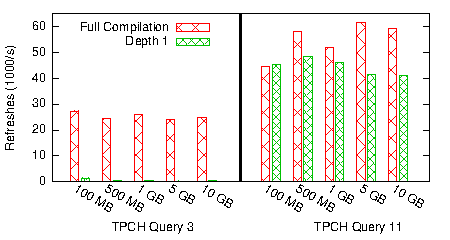
\includegraphics[width=3in]{../graphs/graphs/scaling.pdf} \\
\caption{Performance scaling with respect to dataset size for TPC-H Queries 3 and 11 respectively.  For these queries, performance remains roughly constant as long as sufficient memory is available.}
%The three fastest-running TPC-H queries (3~(b), 11~(c), and 22~(d)) run on a 5GB dataset: (b) Quadratic effects from early parts of the workload become apparent in IVM at this scale, while full compilation remains linear. (c) Maintaining the base relations already projected and aggregated gives a slight edge to full compilation at this scale.  (d) Full compilation performance is reduced due to updates being linear in the size of CUSTOMER, but still performs better than depth 1.
\label{fig:experiments:big}
%\label{fig:experiments:big:tpch3}
%\label{fig:experiments:big:tpch11}
%\label{fig:experiments:big:tpch22}

\end{center}\vspace*{-0.2in}
\end{figure}



